\begin{tabular}{lrrrrrrrrrrrr}
\toprule
BENCHMARK                          & b.sort            &  h.sort           & b.srch            & fft               & xxtea             & md5               & rc5               & coremk            & \makebox[0.2mm]{}   & average           \\
\hline
\multicolumn{10}{l}{CODE SIZE (BYTES)} \\
% Take JVM, Native C and AOT original from results_0BASE_R___P__C0_A0_S0_G1
\xxt JVM                           &                78 &               140 &                91 &               493 &               384 &              2986 &               457 &              5719 &     &                   \\
\xxt Native C                      &               150 &               416 &               212 &              1214 &              1442 &              9458 &               910 &             10388 &     &                   \\
\xxt AOT original                  &               520 &              1170 &               616 &              2694 &              3780 &             29362 &              4074 &             33668 &     &                   \\
% Take AOT optimised from results_4MARK_R11_P7_C1_A1_S1_G1
\xxt AOT optimised                 &               344 &               738 &               450 &              1460 &              2268 &             14798 &              2140 &             25560 &     &                   \\
\hline
\multicolumn{10}{l}{CODE SIZE OVERHEAD BEFORE OPTIMISATIONS (\%)} \\
% Take this from main-code-size-graph.xlsx 
\xxt Total                         &             242.1 &             179.9 &             190.6 &             121.9 &             162.1 &             210.4 &             347.7 &             223.8 &     &             209.8 \\
  \xxxt push/pop                   & \xt          57.9 & \xt          61.2 & \xt          52.8 & \xt          55.7 & \xt         102.6 & \xt         133.1 & \xt         163.1 & \xt          74.5 &     & \xt          87.6 \\
  \xxxt load/store                 & \xt          89.5 & \xt          64.1 & \xt          69.8 & \xt          31.8 & \xt          28.4 & \xt          56.7 & \xt          67.9 & \xt          53.5 &     & \xt          57.7 \\
  \xxxt mov(w)                     & \xt           1.3 & \xt           1.4 & \xt           0.9 & \xt           0.3 & \xt           0.7 & \xt          -2.7 & \xt          -1.3 & \xt           1.4 &     & \xt           0.3 \\
  \xxxt other                      & \xt          93.4 & \xt          53.1 & \xt          67.0 & \xt          34.1 & \xt          30.4 & \xt          23.3 & \xt         118.0 & \xt          94.4 &     & \xt          64.2 \\
\multicolumn{10}{l}{CODE SIZE OVERHEAD REDUCTION PER OPTIMISATION (\%)} \\
\xxt Impr. peephole                &             -57.9 &             -41.1 &             -45.3 &             -26.5 &             -38.5 &             -54.3 &             -62.4 &             -30.7 &     &             -44.6 \\
\xxt Stack caching                 &             -13.1 &             -20.6 &             -24.5 &             -37.1 &             -56.1 &             -78.6 &            -106.4 &             -18.7 &     &             -44.4 \\
\xxt Pop. val. caching             &             -18.5 &             -27.8 &               0.0 &             -13.8 &              -6.2 &             -18.8 &             -17.8 &             -12.6 &     &             -14.4 \\
\xxt Mark loops                    &              -2.6 &              +4.8 &              +7.5 &              -5.9 &              +6.0 &              -1.1 &              -3.7 &              -3.8 &     &               0.2 \\
\xxt Const shift                   &               0.0 &              -2.4 &              -4.7 &              -5.3 &              +1.6 &              +4.0 &              -5.5 &              -1.1 &     &              -1.7 \\
\xxt 16-bit array index            &             -23.7 &             -16.2 &             -11.3 &             -13.0 &             -11.6 &              -5.1 &             -16.7 &              -8.8 &     &             -13.3 \\
\xxt SIMUL                         &               0.0 &               0.0 &               0.0 &               0.0 &               0.0 &               0.0 &               0.0 &              -2.3 &     &              -0.3 \\
\multicolumn{10}{l}{CODE SIZE OVERHEAD AFTER OPTIMISATIONS (\%)} \\
\xxt Total                         &             126.3 &              76.6 &             112.3 &              20.3 &              57.3 &              56.5 &             135.2 &             145.8 &     &              91.3 \\
  \xxxt push/pop                   & \xt          21.1 & \xt           5.7 & \xt           7.5 & \xt           0.0 & \xt          13.3 & \xt           0.0 & \xt           4.4 & \xt          19.4 &     & \xt           8.9 \\
  \xxxt load/store                 & \xt          31.6 & \xt          33.5 & \xt          47.2 & \xt           4.1 & \xt          14.8 & \xt          37.2 & \xt          25.3 & \xt          36.8 &     & \xt          28.8 \\
  \xxxt mov(w)                     & \xt           0.0 & \xt           3.8 & \xt           4.7 & \xt          -2.6 & \xt           2.5 & \xt          -1.8 & \xt          17.8 & \xt           5.4 &     & \xt           3.7 \\
  \xxxt other                      & \xt          73.7 & \xt          33.5 & \xt          52.8 & \xt          18.8 & \xt          26.6 & \xt          21.0 & \xt          87.7 & \xt          84.2 &     & \xt          49.8 \\
\bottomrule
\end{tabular}   


\section{AOT translation: code size}
\label{sec-evaluation-aot-translation-code-size}
Next we examine the effects of our optimisations on code size. Two factors are important here: the size of the VM itself and the size of the code it generates.

The size overhead for the generated code is shown in figures \ref{fig-codesize-per-opcode-category} and \ref{fig-codesize-per-benchmark}, again split up per instruction category and benchmark respectively. For the first three optimisations, the two graphs follow a similar pattern as the performance graphs. These optimisations eliminate the need to emit certain instructions, which reduces code size and improves performance at the same time.

The mark loops optimisation moves loads and stores for pinned variables outside of the loop. This reduces performance overhead by 43\%, but the effect on code size varies per benchmark: some are slightly smaller, others slightly larger.

For each variable that is live at the beginning of the loop, the VM emits the load before the mark loop block, so code size is only reduced if the variable is loaded more than once. Code size may actually increase if the value is then popped destructively, since this causes the VM to emit a \mycode{mov}. Stores follow a similar argument. Also, for small methods the extra registers used may mean we have to save more call-saved registers in the method prologue. Finally, we get the performance advantage for each run-time iteration, but the effect on code size, whether positive or negative, only once.

% \begin{figure}
%  \centering
%  \begin{minipage}{0.45\textwidth}
%   \centering
%   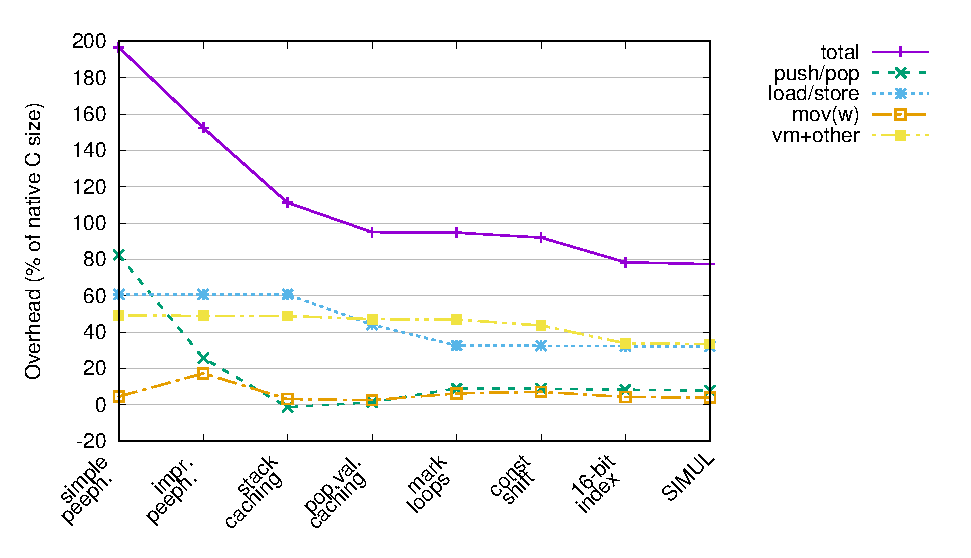
\includegraphics[width=\mygraphsize]{codesizeoverhead-per-opcode-category.eps}
%   \caption{Code size overhead per category}
%   \label{fig-codesize-per-opcode-category}
%  \end{minipage}\hfill
%  \begin{minipage}{0.45\textwidth}
%   \centering
%   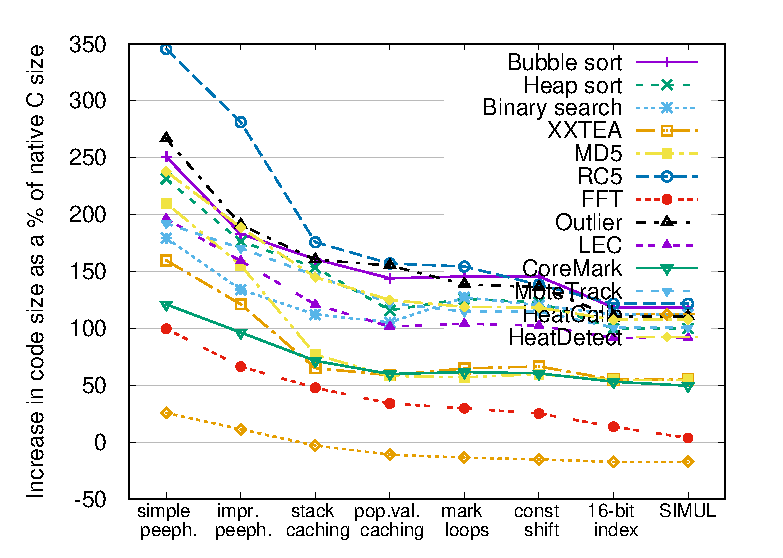
\includegraphics[width=\mygraphsize]{codesizeoverhead-per-benchmark.eps}
%   \caption{Code size overhead per benchmark}
%   \label{fig-codesize-per-benchmark}
%  \end{minipage}
% \end{figure}

\begin{figure}
\centering
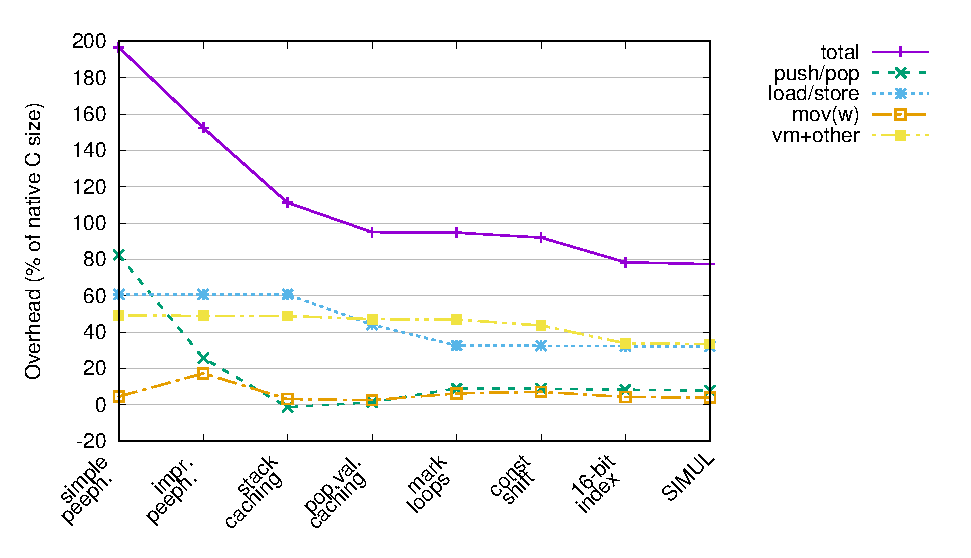
\includegraphics[width=\mygraphsize]{codesizeoverhead-per-opcode-category.eps}
\caption{Code size overhead per category}
\label{fig-codesize-per-opcode-category}
\end{figure}

\begin{figure}
\centering
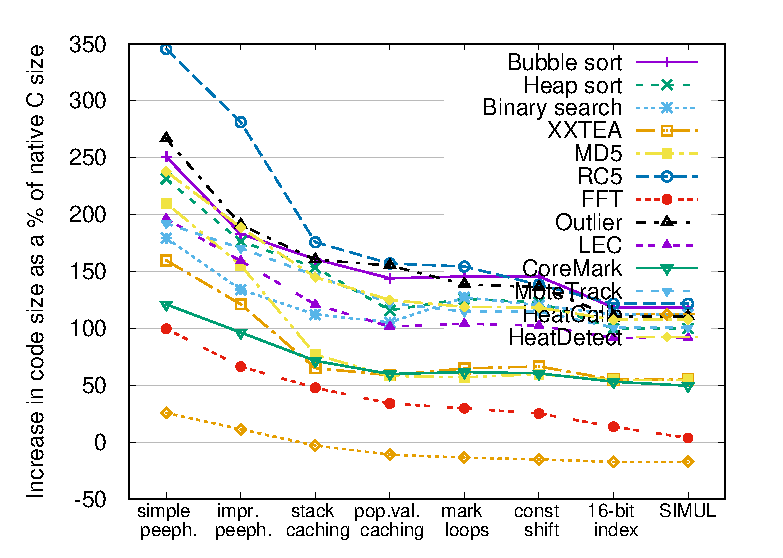
\includegraphics[width=\mygraphsize]{codesizeoverhead-per-benchmark.eps}
\caption{Code size overhead per benchmark}
\label{fig-codesize-per-benchmark}
\end{figure}

The constant shift optimisation unrolls the loop that is normally generated for bit shifts. This significantly improves performance, but the effect on the code size depends on the number of bits to shift by. The constant load and loop take at least 5 instructions. In most cases the unrolled shifts are smaller, but \mybench{MD5} and \mybench{XXTEA} show a small increase in code size since they contains shifts by a large number of bits.

Using 16-bit array indexes also reduces code size. The benchmarks here already have the manual code optimisations, so they use short index variables. This means the infuser emits \mycode{S2I} instructions to cast them to 32-bit ints if the array access instructions expect an int index. Not having to emit those when the array access instructions expect a 16-bit index, and the reduced work the access instruction needs to do, saves 14\% code size overhead in addition to the 19\% reduction in performance overhead. Using 32-bit variables in the source code also removes the need for \mycode{S2I} instructions, but the extra effort needed to manipulate the 32-bit index variable makes the net code size even larger.

\subsection{VM code size and break-even point}
These more complex code generation techniques do increase the size of our compiler. The first column in Table \ref{tbl-code-size-and-memory-consumption} shows the difference in code size between the AOT translator and Darjeeling's interpreter. The basic AOT approach is 6863 B larger than the interpreter, and each optimisation adds a little to the size of the VM.

They also generate significantly smaller code. The third column shows the reduction in the generated code size compared to the baseline approach. Here we show the reduction in total size, as opposed to the overhead used elsewhere, to be able to calculate the break-even point. Using the improved peephole optimiser adds 276 bytes to the VM, but it reduces the size of the generated code by 14.6\%. If we have more than 1.9 KB available to store user programmes, this reduction will outweigh the increase in VM size. Adding more complex optimisations further increases the VM size, but compared to the baseline approach, the break-even point is well within the range of memory typically available on a sensor node, peaking at at most 17.7 KB.

As is often the case, there is a tradeoff between size and performance. The interpreter is smaller than each version of our AOT compiler, and Table \ref{tbl-codesize-per-benchmark} shows bytecode is smaller than both native C and AOT compiled code, but the interpreter's performance penalty may be unacceptable in many cases. Using AOT compilation we can achieve adequate performance, but the most important drawback has been an increase in generated code size. These optimisations help to mitigate this drawback, and both improve performance, and allow us to load more code on a node.

For the smallest devices, or if we want to be able to load especially large programmes, we may decide to use only a selection of optimisations to limit the VM size and still get both a reasonable performance, and most of the code size reduction. For example, dropping the markloop and constant shift optimisations would reduces the size of the VM by 3.7 KB but keeps most of the reduction in generated code size, while performance overhead would increase to about 127\%.

% UPDATED 20180213

\begin{tabular}{lrrrrrr}
\toprule
                          & size vs     & size vs  &                      & AOT code  &   break & memory    \\
                          & interpreter & baseline &                      & reduction &   even  & usage     \\
\midrule
Baseline                  &     6605 B  &          &                      &           &         & 23 B      \\
Improved peephole         &     6881 B  &   276 B  & \scriptsize   (+276) &  -14.8\%  &  1.9 KB & 23 B      \\
Simple stack caching      &     7825 B  &  1220 B  & \scriptsize   (+944) &  -27.6\%  &  4.4 KB & 34 B      \\
Popped value caching      &     9057 B  &  2452 B  & \scriptsize  (+1232) &  -33.1\%  &  7.4 KB & 78 B      \\
Markloop                  &    12337 B  &  5732 B  & \scriptsize  (+3280) &  -33.0\%  & 17.4 KB & 85 B      \\
Const shift               &    12785 B  &  6180 B  & \scriptsize   (+448) &  -33.8\%  & 18.3 KB & 85 B      \\
16-bit array index        &    12765 B  &  6160 B  & \scriptsize    (-20) &  -38.2\%  & 16.1 KB & 85 B      \\
SIMUL                     &    12831 B  &  6226 B  & \scriptsize    (+66) &  -38.7\%  & 16.1 KB & 85 B      \\
Lightweight methods       &    13367 B  &  6762 B  & \scriptsize   (+536) &  -38.9\%  & 17.4 KB & 85 B      \\
\bottomrule
\end{tabular}

\subsection{VM memory consumption} The last column in Table \ref{tbl-code-size-and-memory-consumption} shows the amount of data that needs to be kept in memory while translating a method. We would like our VM to be able to load new code while other tasks are running concurrently. Here we only list the data that the VM would need to maintain in between receiving messages with new code since this is the amount of memory that would not be available to other tasks during this process. Of course new code is being processed, more stack memory is used, but this is freed a batch of instructions has been processed and can be reused by other applications.

For the baseline approach we only use 25 bytes for a number of commonly used values such as a pointer to the next instruction to be compiled, the number of instructions in the method, etc. The simple stack caching approach adds a 11 byte array to store the state of each register pair we use for stack caching. Popped value caching adds two more arrays of 16-bit elements to store the value tag and age of each value. Mark loops only needs an extra 16-bit word to mark which registers are pinned, and a few other variables. Finally, the instruction set optimisations do not require any additional memory. In total, our compiler requires 87 bytes of memory during the compilation process.

